
%% bare_conf.tex
%% V1.3
%% 2007/01/11
%% by Michael Shell
%% See:
%% http://www.michaelshell.org/
%% for current contact information.
%%
%% This is a skeleton file demonstrating the use of IEEEtran.cls
%% (requires IEEEtran.cls version 1.7 or later) with an IEEE conference paper.
%%
%% Support sites:
%% http://www.michaelshell.org/tex/ieeetran/
%% http://www.ctan.org/tex-archive/macros/latex/contrib/IEEEtran/
%% and
%% http://www.ieee.org/

%%*************************************************************************
%% Legal Notice:
%% This code is offered as-is without any warranty either expressed or
%% implied; without even the implied warranty of MERCHANTABILITY or
%% FITNESS FOR A PARTICULAR PURPOSE! 
%% User assumes all risk.
%% In no event shall IEEE or any contributor to this code be liable for
%% any damages or losses, including, but not limited to, incidental,
%% consequential, or any other damages, resulting from the use or misuse
%% of any information contained here.
%%
%% All comments are the opinions of their respective authors and are not
%% necessarily endorsed by the IEEE.
%%
%% This work is distributed under the LaTeX Project Public License (LPPL)
%% ( http://www.latex-project.org/ ) version 1.3, and may be freely used,
%% distributed and modified. A copy of the LPPL, version 1.3, is included
%% in the base LaTeX documentation of all distributions of LaTeX released
%% 2003/12/01 or later.
%% Retain all contribution notices and credits.
%% ** Modified files should be clearly indicated as such, including  **
%% ** renaming them and changing author support contact information. **
%%
%% File list of work: IEEEtran.cls, IEEEtran_HOWTO.pdf, bare_adv.tex,
%%                    bare_conf.tex, bare_jrnl.tex, bare_jrnl_compsoc.tex
%%*************************************************************************

% *** Authors should verify (and, if needed, correct) their LaTeX system  ***
% *** with the testflow diagnostic prior to trusting their LaTeX platform ***
% *** with production work. IEEE's font choices can trigger bugs that do  ***
% *** not appear when using other class files.                            ***
% The testflow support page is at:
% http://www.michaelshell.org/tex/testflow/



% Note that the a4paper option is mainly intended so that authors in
% countries using A4 can easily print to A4 and see how their papers will
% look in print - the typesetting of the document will not typically be
% affected with changes in paper size (but the bottom and side margins will).
% Use the testflow package mentioned above to verify correct handling of
% both paper sizes by the user's LaTeX system.
%
% Also note that the "draftcls" or "draftclsnofoot", not "draft", option
% should be used if it is desired that the figures are to be displayed in
% draft mode.
%
\documentclass[conference]{IEEEtran}
% Add the compsoc option for Computer Society conferences.
%
% If IEEEtran.cls has not been installed into the LaTeX system files,
% manually specify the path to it like:
% \documentclass[conference]{../sty/IEEEtran}
% Some very useful LaTeX packages include:
% (uncomment the ones you want to load)

% *** MISC UTILITY PACKAGES ***
%
%\usepackage{ifpdf}
% Heiko Oberdiek's ifpdf.sty is very useful if you need conditional
% compilation based on whether the output is pdf or dvi.
% usage:
% \ifpdf
%   % pdf code
% \else
%   % dvi code
% \fi
% The latest version of ifpdf.sty can be obtained from:
% http://www.ctan.org/tex-archive/macros/latex/contrib/oberdiek/
% Also, note that IEEEtran.cls V1.7 and later provides a builtin
% \ifCLASSINFOpdf conditional that works the same way.
% When switching from latex to pdflatex and vice-versa, the compiler may
% have to be run twice to clear warning/error messages.

% *** CITATION PACKAGES ***
%
\usepackage{cite}
% cite.sty was written by Donald Arseneau
% V1.6 and later of IEEEtran pre-defines the format of the cite.sty package
% \cite{} output to follow that of IEEE. Loading the cite package will
% result in citation numbers being automatically sorted and properly
% "compressed/ranged". e.g., [1], [9], [2], [7], [5], [6] without using
% cite.sty will become [1], [2], [5]--[7], [9] using cite.sty. cite.sty's
% \cite will automatically add leading space, if needed. Use cite.sty's
% noadjust option (cite.sty V3.8 and later) if you want to turn this off.
% cite.sty is already installed on most LaTeX systems. Be sure and use
% version 4.0 (2003-05-27) and later if using hyperref.sty. cite.sty does
% not currently provide for hyperlinked citations.
% The latest version can be obtained at:
% http://www.ctan.org/tex-archive/macros/latex/contrib/cite/
% The documentation is contained in the cite.sty file itself.

% *** GRAPHICS RELATED PACKAGES ***
%
\ifCLASSINFOpdf
  % \usepackage[pdftex]{graphicx}
  % declare the path(s) where your graphic files are
  % \graphicspath{{../pdf/}{../jpeg/}}
  % and their extensions so you won't have to specify these with
  % every instance of \includegraphics
  % \DeclareGraphicsExtensions{.pdf,.jpeg,.png}
\else
  % or other class option (dvipsone, dvipdf, if not using dvips). graphicx
  % will default to the driver specified in the system graphics.cfg if no
  % driver is specified.
  \usepackage[dvips]{graphicx}
  % declare the path(s) where your graphic files are
  \graphicspath{{../fig/}}
  % and their extensions so you won't have to specify these with
  % every instance of \includegraphics
  % \DeclareGraphicsExtensions{.eps}
\fi
% graphicx was written by David Carlisle and Sebastian Rahtz. It is
% required if you want graphics, photos, etc. graphicx.sty is already
% installed on most LaTeX systems. The latest version and documentation can
% be obtained at: 
% http://www.ctan.org/tex-archive/macros/latex/required/graphics/
% Another good source of documentation is "Using Imported Graphics in
% LaTeX2e" by Keith Reckdahl which can be found as epslatex.ps or
% epslatex.pdf at: http://www.ctan.org/tex-archive/info/
%
% latex, and pdflatex in dvi mode, support graphics in encapsulated
% postscript (.eps) format. pdflatex in pdf mode supports graphics
% in .pdf, .jpeg, .png and .mps (metapost) formats. Users should ensure
% that all non-photo figures use a vector format (.eps, .pdf, .mps) and
% not a bitmapped formats (.jpeg, .png). IEEE frowns on bitmapped formats
% which can result in "jaggedy"/blurry rendering of lines and letters as
% well as large increases in file sizes.
%
% You can find documentation about the pdfTeX application at:
% http://www.tug.org/applications/pdftex

% *** MATH PACKAGES ***
%
\usepackage[cmex10]{amsmath}
% A popular package from the American Mathematical Society that provides
% many useful and powerful commands for dealing with mathematics. If using
% it, be sure to load this package with the cmex10 option to ensure that
% only type 1 fonts will utilized at all point sizes. Without this option,
% it is possible that some math symbols, particularly those within
% footnotes, will be rendered in bitmap form which will result in a
% document that can not be IEEE Xplore compliant!
%
% Also, note that the amsmath package sets \interdisplaylinepenalty to 10000
% thus preventing page breaks from occurring within multiline equations. Use:
\interdisplaylinepenalty=2500
% after loading amsmath to restore such page breaks as IEEEtran.cls normally
% does. amsmath.sty is already installed on most LaTeX systems. The latest
% version and documentation can be obtained at:
% http://www.ctan.org/tex-archive/macros/latex/required/amslatex/math/

% *** SPECIALIZED LIST PACKAGES ***
%
%\usepackage{algorithmic}
% algorithmic.sty was written by Peter Williams and Rogerio Brito.
% This package provides an algorithmic environment fo describing algorithms.
% You can use the algorithmic environment in-text or within a figure
% environment to provide for a floating algorithm. Do NOT use the algorithm
% floating environment provided by algorithm.sty (by the same authors) or
% algorithm2e.sty (by Christophe Fiorio) as IEEE does not use dedicated
% algorithm float types and packages that provide these will not provide
% correct IEEE style captions. The latest version and documentation of
% algorithmic.sty can be obtained at:
% http://www.ctan.org/tex-archive/macros/latex/contrib/algorithms/
% There is also a support site at:
% http://algorithms.berlios.de/index.html
% Also of interest may be the (relatively newer and more customizable)
% algorithmicx.sty package by Szasz Janos:
% http://www.ctan.org/tex-archive/macros/latex/contrib/algorithmicx/

% *** ALIGNMENT PACKAGES ***
%
%\usepackage{array}
% Frank Mittelbach's and David Carlisle's array.sty patches and improves
% the standard LaTeX2e array and tabular environments to provide better
% appearance and additional user controls. As the default LaTeX2e table
% generation code is lacking to the point of almost being broken with
% respect to the quality of the end results, all users are strongly
% advised to use an enhanced (at the very least that provided by array.sty)
% set of table tools. array.sty is already installed on most systems. The
% latest version and documentation can be obtained at:
% http://www.ctan.org/tex-archive/macros/latex/required/tools/

%\usepackage{mdwmath}
%\usepackage{mdwtab}
% Also highly recommended is Mark Wooding's extremely powerful MDW tools,
% especially mdwmath.sty and mdwtab.sty which are used to format equations
% and tables, respectively. The MDWtools set is already installed on most
% LaTeX systems. The lastest version and documentation is available at:
% http://www.ctan.org/tex-archive/macros/latex/contrib/mdwtools/

% IEEEtran contains the IEEEeqnarray family of commands that can be used to
% generate multiline equations as well as matrices, tables, etc., of high
% quality.

%\usepackage{eqparbox}
% Also of notable interest is Scott Pakin's eqparbox package for creating
% (automatically sized) equal width boxes - aka "natural width parboxes".
% Available at:
% http://www.ctan.org/tex-archive/macros/latex/contrib/eqparbox/

% *** SUBFIGURE PACKAGES ***
\usepackage[tight,footnotesize]{subfigure}
% subfigure.sty was written by Steven Douglas Cochran. This package makes it
% easy to put subfigures in your figures. e.g., "Figure 1a and 1b". For IEEE
% work, it is a good idea to load it with the tight package option to reduce
% the amount of white space around the subfigures. subfigure.sty is already
% installed on most LaTeX systems. The latest version and documentation can
% be obtained at:
% http://www.ctan.org/tex-archive/obsolete/macros/latex/contrib/subfigure/
% subfigure.sty has been superceeded by subfig.sty.

%\usepackage[caption=false]{caption}
%\usepackage[font=footnotesize]{subfig}
% subfig.sty, also written by Steven Douglas Cochran, is the modern
% replacement for subfigure.sty. However, subfig.sty requires and
% automatically loads Axel Sommerfeldt's caption.sty which will override
% IEEEtran.cls handling of captions and this will result in nonIEEE style
% figure/table captions. To prevent this problem, be sure and preload
% caption.sty with its "caption=false" package option. This is will preserve
% IEEEtran.cls handing of captions. Version 1.3 (2005/06/28) and later 
% (recommended due to many improvements over 1.2) of subfig.sty supports
% the caption=false option directly:
%\usepackage[caption=false,font=footnotesize]{subfig}
%
% The latest version and documentation can be obtained at:
% http://www.ctan.org/tex-archive/macros/latex/contrib/subfig/
% The latest version and documentation of caption.sty can be obtained at:
% http://www.ctan.org/tex-archive/macros/latex/contrib/caption/

% *** FLOAT PACKAGES ***
%
%\usepackage{fixltx2e}
% fixltx2e, the successor to the earlier fix2col.sty, was written by
% Frank Mittelbach and David Carlisle. This package corrects a few problems
% in the LaTeX2e kernel, the most notable of which is that in current
% LaTeX2e releases, the ordering of single and double column floats is not
% guaranteed to be preserved. Thus, an unpatched LaTeX2e can allow a
% single column figure to be placed prior to an earlier double column
% figure. The latest version and documentation can be found at:
% http://www.ctan.org/tex-archive/macros/latex/base/

%\usepackage{stfloats}
% stfloats.sty was written by Sigitas Tolusis. This package gives LaTeX2e
% the ability to do double column floats at the bottom of the page as well
% as the top. (e.g., "\begin{figure*}[!b]" is not normally possible in
% LaTeX2e). It also provides a command:
%\fnbelowfloat
% to enable the placement of footnotes below bottom floats (the standard
% LaTeX2e kernel puts them above bottom floats). This is an invasive package
% which rewrites many portions of the LaTeX2e float routines. It may not work
% with other packages that modify the LaTeX2e float routines. The latest
% version and documentation can be obtained at:
% http://www.ctan.org/tex-archive/macros/latex/contrib/sttools/
% Documentation is contained in the stfloats.sty comments as well as in the
% presfull.pdf file. Do not use the stfloats baselinefloat ability as IEEE
% does not allow \baselineskip to stretch. Authors submitting work to the
% IEEE should note that IEEE rarely uses double column equations and
% that authors should try to avoid such use. Do not be tempted to use the
% cuted.sty or midfloat.sty packages (also by Sigitas Tolusis) as IEEE does
% not format its papers in such ways.

% *** PDF, URL AND HYPERLINK PACKAGES ***
%
\usepackage{url}
% url.sty was written by Donald Arseneau. It provides better support for
% handling and breaking URLs. url.sty is already installed on most LaTeX
% systems. The latest version can be obtained at:
% http://www.ctan.org/tex-archive/macros/latex/contrib/misc/
% Read the url.sty source comments for usage information. Basically,
% \url{my_url_here}.

% *** Do not adjust lengths that control margins, column widths, etc. ***
% *** Do not use packages that alter fonts (such as pslatex).         ***
% There should be no need to do such things with IEEEtran.cls V1.6 and later.
% (Unless specifically asked to do so by the journal or conference you plan
% to submit to, of course. )

\usepackage{multirow}
\usepackage{tikz}

% correct bad hyphenation here
\hyphenation{op-tical net-works semi-conduc-tor}

\newcommand{\eqdef}{\overset{\mathrm{def}}{=\joinrel=}}

\begin{document}
%
% paper title
% can use linebreaks \\ within to get better formatting as desired
\title{Real-Time Continuous Gesture Recognition for Natural Human-Centric
Interaction }

% author names and affiliations
% use a multiple column layout for up to three different
% affiliations
\author{\IEEEauthorblockN{Ying Yin}
\IEEEauthorblockA{CSAIL MIT\\
Email: yingyin@csail.mit.edu}
\and
\IEEEauthorblockN{Randall Davis}
\IEEEauthorblockA{CSAIL MIT\\
Email: davis@csail.mit.edu}
}

% conference papers do not typically use \thanks and this command
% is locked out in conference mode. If really needed, such as for
% the acknowledgment of grants, issue a \IEEEoverridecommandlockouts
% after \documentclass

% for over three affiliations, or if they all won't fit within the width
% of the page, use this alternative format:
% 
%\author{\IEEEauthorblockN{Michael Shell\IEEEauthorrefmark{1},
%Homer Simpson\IEEEauthorrefmark{2},
%James Kirk\IEEEauthorrefmark{3}, 
%Montgomery Scott\IEEEauthorrefmark{3} and
%Eldon Tyrell\IEEEauthorrefmark{4}}
%\IEEEauthorblockA{\IEEEauthorrefmark{1}School of Electrical and Computer Engineering\\
%Georgia Institute of Technology,
%Atlanta, Georgia 30332--0250\\ Email: see http://www.michaelshell.org/contact.html}
%\IEEEauthorblockA{\IEEEauthorrefmark{2}Twentieth Century Fox, Springfield, USA\\
%Email: homer@thesimpsons.com}
%\IEEEauthorblockA{\IEEEauthorrefmark{3}Starfleet Academy, San Francisco, California 96678-2391\\
%Telephone: (800) 555--1212, Fax: (888) 555--1212}
%\IEEEauthorblockA{\IEEEauthorrefmark{4}Tyrell Inc., 123 Replicant Street, Los Angeles, California 90210--4321}}

% make the title area
\maketitle

\begin{abstract}
%\boldmath
We have developed a real-time continuous gesture recognition system that handles two types of gestures seamlessly: 
ones that are characterized by their dynamic paths and ones that are characterized by their static hand poses. 
We design the system based on previous user studies on natural interaction, and
thus are able to address problems that are previously neglected. Our
probabilistic based recognition framework unifies the recognition of the two
types gestures. We use information from the hidden states in the hidden Markov
model to identify the different phases in a gesture: the pre-stroke, the nucleus
and the post-stroke phases. This allows the system to respond appropriately
according different gestures that require discrete or continuous responses. Our
system explores more potential with human gestures rather than just making
the hand function as a mouse. We also collected a new gesture data set that
contains the two types of gestures, and propose a new performance metric that
is relevant for evaluating gesture recognition methods for real-time
interaction.
The system is also extensible. Users can define their own gestures by
giving a few examples rather than writing code. Adding a new gesture only takes
a couple of minutes.

\end{abstract}
% IEEEtran.cls defaults to using nonbold math in the Abstract.
% This preserves the distinction between vectors and scalars. However,
% if the conference you are submitting to favors bold math in the abstract,
% then you can use LaTeX's standard command \boldmath at the very start
% of the abstract to achieve this. Many IEEE journals/conferences frown on
% math in the abstract anyway.

% no keywords




% For peer review papers, you can put extra information on the cover
% page as needed:
% \ifCLASSOPTIONpeerreview
% \begin{center} \bfseries EDICS Category: 3-BBND \end{center}
% \fi
%
% For peerreview papers, this IEEEtran command inserts a page break and
% creates the second title. It will be ignored for other modes.
\IEEEpeerreviewmaketitle

\section{Introduction}
% no \IEEEPARstart
\begin{quotation}
Imagine next time when you make a presentation, you do not need to stand close
to your laptop or use a remote control with limited functionality. You can
present your work naturally as having a conversation with your audience. You
swipe your hand left and right to change slides. When you point to the slide
with your hand, the display shows a pointer cursor following where you are
pointing at. When you are showing a video,
you use a palm forward hand pose and move left and right to fast forward or
rewind the video. You can also say ``faster'' or ``slower'' to change the speed
of the process. When you need to jump to a particular slide, you make a circle
gesture to show all the slides and point to the slide and say ``show this
slide'' to display that slide. You can also make a dismiss gesture to pause the
slide show (making the screen black) to take the distracting slides off the
screen and get full attention from the audience during presentation.
\end{quotation}

The scenario above shows an application of multi-modal interface to a real-world
problem. Different types of gestures play an important part in the scenario.

Recent advancement in sensing technology (depth sensors, the Leap Motion sensor)
and computer vision (skeleton tracking \cite{shotton13}) have brought on new
possibilities in interaction techniques that depart from the traditional mouse
and keyboard that have been used for decades. However, many gestural interfaces
still mainly make the hands function as a mouse to interact with the interface
with a limited number of other gestures. Previous research on gesture
recognition usually focuses on one form of gesture and the evaluation is also
offline. We believe that for designing a gesture recognition system, we need to
start from the user interaction perspective. What are the different types of
gestures we need to recognize, when should the system respond and how should the
model be trained or defined. Hence we developed our system from a human-centric
approach.

Contributions:
\begin{itemize}
  \item A unified probabilistic framework for real-time gesture recognition that
  combines two forms of gestures.
  \item Use embedded training and hidden state information to detect different
  gesture phase and allow the system to respond more promptly.
  \item Collect a new dataset that include two forms of gesture that are
  currently lacking in the community and propose a evaluation metric that is
  pertinent to real-time interaction and different types of gestures.
\end{itemize}

\section{Gesture Taxonomy for Natural Interaction}\label{sec:taxonomy}
Several gesture taxonomies have been suggested in the literature. Some of them
deal with psychological aspects of gestures \cite{kendon86, mcneill82}, while
some of them deal directly with human computer interaction (HCI) \cite{quek94,
quek95, Pavlovic97}. The taxonomy that seems most appropriate for natural HCI
and human-centric design was developed Wobbrock et al. \cite{wobbrock09}. Their
study is based on eliciting natural behavior from non-technical users when
interacting with a computing system. Although their user study focuses on
tabletop gestures, we believe that the results can be generalized to other
interactive interfaces, e.g., vertical displays. The results from Wobbrock et
al. not only give guidance to gesture set design, but also guidance to the
gesture recognition technology and this is what we are addressing.

Wobbrock et al. classifies gestures in four orthogonal dimensions. As a first
step, we focus on two of them and incorporate them in designing the
gesture recognition system and interface. We also further generalize the
taxonomy to encompass interaction for both vertical and horizontal displays.

One dimension is the \textit{form} of a gesture. There are two main categories
in this dimension that are important to distinguish. One category of gestures are characterized
by their distinctive paths but they do not have distinct hand poses. For
example, a \textit{swipe left} gesture is characterized by the right to left motion, and a \textit{circle} gesture is
characterized by the circular motion of the hand. Typically users just
hold their hand in some natural relaxed poses. Another category of gestures are
characterized by their distinctive hand poses but users may move the hand in any
directions, i.e., no distinct paths. This category of gestures are usually
associated with direct manipulation of some virtual objects on the interface.
For example, a user may use a \textit{point} hand pose and move around to point at different things on a display; or a user can use a \textit{palm forward} hand pose to signal direct
control of a video and move the hand to fast forward or rewind the video. 

\begin{table}[t]
\caption{Taxonomy of gestures for natural interaction.}
\label{tab:taxonomy}
\centering
\begin{tabular}{|c|l|l|}
\hline
\multirow{2}{*}{\textbf{\textit{Form}}} & \textit{distinct path} & with any hand
pose
\\
\cline{2-3} 
                               & \textit{distinct hand pose} & with any path \\
\hline
\multirow{2}{*}{\textbf{\textit{Flow}}} & \textit{discrete} & response occurs
\textit{after} the user acts \\
\cline{2-3}
              & \textit{continuous} & response occurs \textit{while} the user
              acts \\
\hline
\end{tabular}
\end{table}

Another dimension is the \textit{flow} of a gesture. A gesture's flow is
discrete if the gesture is performed, delimited, recognized, and responded to
as an \textit{event}. An example is the \textit{wave} gesture which has a few
repetitions of left and right movement and usually we want the system to respond
at the last repetition. Flow is continuous if ongoing recognition is required
and the system should respond frame by frame, such as during the
\textit{pointing} gesture, we want to show the cursor on the screen continuously
move according to the hand position. Hence, the flow of the gesture affects how
the system should respond and this can be a choice at the application level. For
the same gesture, the application can choose to respond in a continuous or
discrete manner. 

\subsection{Temporal Modeling of Gestures}
To build a real-time interactive system, it is important to have a responsive
system that respond to users' gesture input appropriately according the flow of
the gesture. As a result, it is important to consider the temporal
characteristics of gestures.

It has been established that three phases make a gesture:
\begin{itemize}
  \item pre-stroke,
  \item nucleus (peak \cite{mcneill82}), and
  \item post-stroke \cite{Pavlovic97}.
\end{itemize}
The three temporal phases are distinguishable through the general hand/arm
motion: ``pre-stroke'' and ``post-stroke'' are movement from and to the
rest position, characterized by the rapid change in the position of the hand.
The ``nucleus'', in general, exhibits relatively slower hand motion. The ``nucleus'' of a gesture,
as Kendon \cite{kendon86} observes, has some ``definite form and enhanced dynamic
qualities''. Every gesture must have a ``nucleus'', which is considered by
Kendon to be the content-carrying part of the gesture. Based on this theory, we
expect that the lack of the ``nucleus'' part is how unintentional movements can
be distinguished from gestures. 

Since ``nucleus'' is the meaningful part of the gesture, for a discrete flow
gesture, we want the system to respond immediately at the end of the ``nucleus''
phase instead of at the end of the ``post-stroke'' phase which can be more
easily detected by finding the start of the rest position. However, in order to
make the system more responsive, we address the more challenging problem of
detecting the start and end of the ``nucleus'' phase from the ``pre-stroke''
and ``post-stroke'' phases. This allows the system to respond to continuous flow
gesture immediately at the start of the ``nucleus'' phase and to discrete flow
gesture at the end of the ``nucleus'' phase.

\subsection{Implications for Gesture Recognition Technology}


\begin{figure}[!t]
\centering
\includegraphics[width=\columnwidth]{fig/system_overview.ps}
\caption{System overview.}
\label{fig:system}
\end{figure}

Gesture label, gesture phase and gesture event information, together with
smoothed hand position information are sent to the application level at each
time frame.

\section{Related Work}\label{sec:related}
There are some previous work that looked at different types of gestures. The
Chalearn Gesture Dataset (CGD 2011) \cite{guyon13} contains a nine gesture categories corresponding to various settings and application domains. It
contains both static postures and dynamic gestures. In this dataset, a static
posture is one in which a single posture is held for a certain duration. In
terms of the static hand posture, the hand is held at similar position for
multiple instance of the same gesture. In this case, the
static postures also have distinct paths so they are likely to be able to
handled by the same method as the dynamic gestures. The gesture recognition
algorithm employed by the top winner is a Bayesian network similar to the hidden
Markov model (HMM) used in speech recognition \cite{guyon13results}. Hence in
this dataset, it does not contain gestures with distinct hand poses but
arbitrary movement. And for this form of gestures, we believe we cannot just
treat them exactly the same as gestures with distinct paths. Because if we train
a model based on the training data that also models the paths, that model may
not be applicable for testing because the movement of the hand can change all
the time.

Keskin et al. \cite{keskin12} proposed a unified framework to allow concurrent
usage of hand gestures, shapes and hand skeletons. Hand gestures are modeled
with mixture of HMMs using spectral clustering. Hand shape classification and
hand skeleton estimation are based on randomized decision forests. Hand
gesture classification is active all the time. The framework estimates a set of
posteriors for the hand shape label at each frame, and continuously use these
posteriors and the velocity vector as observation to spot and classify known
gestures. They distinguish gestures with pure motion and pure hand shape by
thresholding the magnitude of the velocity vector. However they did mention
handling gestures with distinct hand poses but with arbitrary movement.

\cite{Oka02}

Most previous work on gesture recognition focus on one form of gestures.
\subsection{Gesture with Distinct Hand Poses}
This group work focus on classifying a set of predefined static hand
poses frame by frame. Freeman and Roth \cite{freeman95} use histogram of local
orientations, a precursor of HOGs for hand pose recognition. Recognition is based on selecting the feature vector in the training set that is closest to the test feature
vector. Suryanarayan et al. \cite{suryanarayan2010} uses a volumetric shape
descriptor computed from depth data as the feature vector and use Support
Vector Machine (SVM) for classification.

\subsection{Gesture with Distinct Paths}
The gesture production process has a direct analogy to the
speech production process \cite{Kettebekov01}, and as a result many previous
work have used HMM for gesture recognition with distinct paths
\cite{Starner95, sharma00}. More recently, the discriminative models such as
conditional random fields (CRF) and its variants hidden CRF \cite{wang06}
and latent dynamic CRF (LDCRF) \cite{morency07} have also been applied to
gesture recognition.
However the discriminative models may require more data to train \cite{ng02} and also may take more time to train
as the parameter space of the model is larger because unlike the generative
model where the parameters are conditional probabilities, there is no such
restriction for the discriminative models.

LDCR also learns the transition parameters between gestures. In our case, we
believe the transition between gestures for interaction is more arbitrary,
unlike for example in sign language, and we assume the transitions between
gestures are uniform and do not need to be trained. 

The generative model (i.e., HMM) allows us to concatenate the trained HMM based
on certain probability assumption. However we cannot the same for the trained
LDCRF models.

\subsection{Online Recognition}
Song et al. uses LDCRF with a temporal sliding window to perform
online sequence labeling and segmentation simultaneously \cite{song12}. Sliding
window method has also been, size of the sliding window, what happens when the window is covers partial parts of a gesture.

\subsection{Commercial Systems}
For example, the Kinect-based
Xbox interaction detects the wave gesture

Leap Motion

\subsection{Data Sets}
Song NATOPS

\section{Hand Tracking and Feature Extraction}
As one form of the gestures are characterized by their distinct hand poses, we
need to track the full hand, rather than just treating the hand as one point. We
also need to derive a feature vector that represents the hand shape as well.

We choose to use the Kinect sensor because we can derive hand shape features
from the depth or RGB data. The skeleton tracking from the Kinect SDK is
relative robust for standing articulated body poses. At each time frame, we use
the hand joint position reported from the SDK to find the initial rough estimation of the
bounding box of the hand in the depth frame. Then we use skin detection to
filter out non-skin pixels in the bounding box after aligning the RGB and the
depth frames, and refine the bounding box using 4 interactions of CAMSHIFT
\cite{bradski98}. We normalize the bounding box to a $32\times 32$ px depth
mapped image. Histogram of oriented gradients (HOGs) \cite{dalal05} is computed from
the normalized hand image (cell size = 4, number of orientation bins = 9). We
only use one fold of normalization to speed up processing and since the depth
data is not affected significantly by lighting conditions. This gives us a
HOG feature of length 441 ($(32/4 - 1)\times (32/4 - 1)\times 9$). The HOG
feature has been used as a hand pose descriptor in previous works \cite{song12} where they are often used as the input to a classifier such as Support Vector Machine
(SVM). Here, after applying principal component analysis (PCA) to reduce the
dimensionality from 441 to 14, we use it directly as part of the input feature
vector to the hidden Markov model (HMM) based recognition framework.

\begin{figure}[!t]
\centering
\includegraphics[width=\columnwidth]{fig/hand_tracking.ps}
\caption{Hand tracking and hand pose feature extraction.}
\label{fig:tracking}
\end{figure}

The feature vector $\underline{x}_t$ at frame $t$ to the recognition
module is then a concatenation of motion features and encoded HOG features. The
motion features include relative position of the hand to the shoulder joint,
velocity and and acceleration, all in 3D world coordinate. The feature vector is
computed for each input frame streamed from the sensor to form a sequence of
feature vectors.

\section{Real-Time Continuous Gesture Recognition}
The temporal model of gestures can be represented by a stochastic state machine.
Each gesture phase can again be represented by a stochastic state machine with
each state generating an observation (i.e. the feature vector). This process
can be viewed as a hierarchical hidden Markov model. If we assume that the
states in the sub-HMMs are not shared, we can collapse the hierarchical HMM
into a one-level HMM. 

\begin{figure}[!t]
\centering
\includegraphics[width=\columnwidth]{fig/hhmm.ps}
\caption{State transition diagram of the hierarchical HMM representation of
gesture phases. Double-ringed states are end states.}
\label{fig:hhmm}
\end{figure}

\begin{figure}[!t]
\centering
\includegraphics[width=\columnwidth]{fig/embedded.ps}
\caption{Embed phase HMMs into an entire gesture.}
\label{fig:embed}
\end{figure}

If we have ground truth labels for the pre-stroke, the nucleus and the
post-stroke phases, we can train the sub-HMMs for each phase and each gesture
separately and then combine them \cite{yin13}. However in practice, for example
if we want users to be able to easily add their new gestures by giving a few
examples, it will be tedious to manually label the start and end of the
three phases. In this case, we can do embedded training \cite{young1994}, i.e.
train each phase HMM embedded in an entire gesture segment (\ref{fig:embed}).
Baum-Welch algorithm can then be used to estimate the transition and emission
parameters.

Through cross-validation, we choose to use one hidden state for pre-stroke and
post-stroke phases. We use the Bakis (left-right) model \cite{Bauer00} for the
nucleus phase, but add a backward transition from the last hidden state to the first
one for gestures with arbitrary number of repetitions (e.g., \textit{wave}
gesture).

We use mixture of Gaussians to model the emission probabilities for each hidden
state. 

\subsection{Unified Framework}
We do not treat the two \textit{forms} of gestures separately: gestures with
distinct paths and gestures with distinct hand poses. Doing that will require
classifying the gestures into the two categories and applying different methods
to further classify the gestures. We want to avoid making early hard decisions
which will be hard to correct. Instead, we want to make decision only when a
response is needed according to the flow of the current most likely gesture and
keep and propagate estimates as probabilities as time progresses.

We incorporate the gestures with distinct hand poses into the HMM-based
framework and use one hidden state to represent their nuclei phases. The
rationale for this is that the hidden state actually represents the hand pose of
the gesture. The variance of the motion features in the mixture of Gaussians
corresponding to the hidden state will be large so that the motion features do
not affect the emission probability very much.

Let $s_{\text{pose}}$ be the single hidden state for the nucleus phase for a
gesture with distinct hand pose. Instead of doing embedded training, we directly
compute the maximum likelihood estimates for the mixture of Gaussians emission
probabilities for $s_{\text{pose}}$. Let $\underline{x}_1^L$ be a sequence of
feature vectors corresponding to a gesture with a distinct hand pose. The
feature vector sequence also contains variations in the hand movement path. We
use Expectation Maximization to estimate the means, covariance matrices and
mixture probabilities for the mixture of Gaussians for this state.

Since there is only one hidden state for $s_{\text{pose}}$, its transition
probability is 1. Its termination probability is estimated according to the
expected duration of the gesture. The self-arc on a state in an HMM defines a 
geometric distribution over waiting time \cite{murphy02}. In the case of the
single state HMM, the probability of remaining in state $s_{\text{pose}}$ for
exactly $d$ steps is $P(d) = p(1-p)^{d - 1}$, where $p = P(END|s_\text{pose})$
is the termination probability for $s_{\text{pose}}$. This means the expected
number of steps remaining in state $s_{\text{pose}}$ is $\frac{1}{p}$. We assume
that the minimum duration of a gesture with distinct hand pose is 1s (30
frames). The termination probability $P(END|s_\text{pose})$ should then set to
be less than $1/30$.

\begin{figure}[t]
\centering
\includegraphics[width=\columnwidth]{fig/single_state.ps}
\end{figure}

For gestures with distinct paths, we use embedded training to combine the three
gesture phases together and use normal Baum-Welch algorithm to compute the
maximum likelihood of the parameters. We also estimate the termination
probabilities as in \cite{yin13}.

We also use one hidden state to model the rest position in a similar way.

\subsection{Real-Time Recognition}
We train the HMMs separately for each gesture, and then combine them into the
hierarchical structure shown in Fig.. We allow sharing of the hidden states for
pre-stroke and post-stroke phases for all the gestures.

The hierarchical model allows us to do simultaneous segmentation and
recognition. We want to avoid doing segmentation first and then find the most
likely HMM for the give sequence. This is because segmentation based on
differentiating rest position versus non-rest position will not allow the system
to respond fast enough as we want the system to respond at the beginning of the
post-stroke phase rather then at the beginning of the rest position. In
addition, making a hard decision on segmentation can also introduce errors that
cannot be corrected. 

For fast inference, we
flatten the hierarchical HMM into a regular HMM by creating an HMM state for
every leaf in the HHMM state transition diagram \cite{murphy02}. Each
hidden state $s_{GPN}$ in the flattened HMM can be indexed by three variables:
$G$ the gesture it belongs to, $P$ the phase it belongs to, and $N$ its position
in the left-right model. For example hidden state $s_{1n2}$ represents the
second hidden state in the nucleus phase of gesture 1.

\begin{figure}[t]
\centering
\includegraphics[width=\columnwidth]{fig/combined.ps}
\caption{Hierarchical HMMs for all gestures.}
\label{fig:combined}
\end{figure}

\subsection{Online Inference}
Once we have a trained model, we use fixed-lag smoothing \cite{murphy02} to do
online inference on the flattened HMM for real-time gesture recognition.
Fixed-lag smoothing is a modified forward-backward algorithm. Unlike online
filtering, which estimates the belief state at current time $t$ using forward
pass, we estimate the state at $t - L$, given all the evidence up to to the
current time $t$, i.e., compute $\gamma_{t - L}(s) \eqdef P(S_{t -
L} = s|\underline{x}_1^t)$, where $L>0$ is the lag. Introducing lag time is a
tradeoff between accuracy and responsiveness. Using some future evidence to
smooth the estimate can increase the accuracy while adding some delay. However
if the delay is small, it might be unnoticeable. We set $L=5$ frames which
$1/6^{th}$ of a second with 30Hz frame rate. (human reaction time)

Fixed-lag smoothing can be implemented efficiently. We compute forward
probabilities $\alpha_t$ normally and keep a history window of $\alpha_{t -
L}\ldots\alpha_t$. At every time frame, we compute backward probabilities
$\beta$ from current time $t$ to $t - L$. Then we can compute
\begin{align}
\gamma_{t - L} = \alpha_{t - L} \cdot \beta_{t - L}
\end{align}  
The time complexity at each time frame is $O(N_s^2L)$ where $N_s$ is the total
number of hidden states in the flattened HMM.

Note that at time $t$, the belief state (define or use probabilities all the
way) at $t - L$ is committed, while the belief state from $t - L + 1$ to $t$ will still be revised later.

Then we can compute the most likely hidden state at $t - L$:
\begin{align}
\hat{s} = \arg\max_s \gamma_{t - L}(s)
\end{align}

From the most likely hidden state, we can map it back to the gesture label it
belongs to, including the rest position and also the gesture phase. In this way
we achieve simultaneous segmentation and recognition.

Gesture events are detected at the boundary of phase change: start pre-stroke,
start gesture nucleus and start post-stroke. This information, together with the
gesture label for the nucleus phase, are sent to the application level.

\begin{figure}[t]
\centering
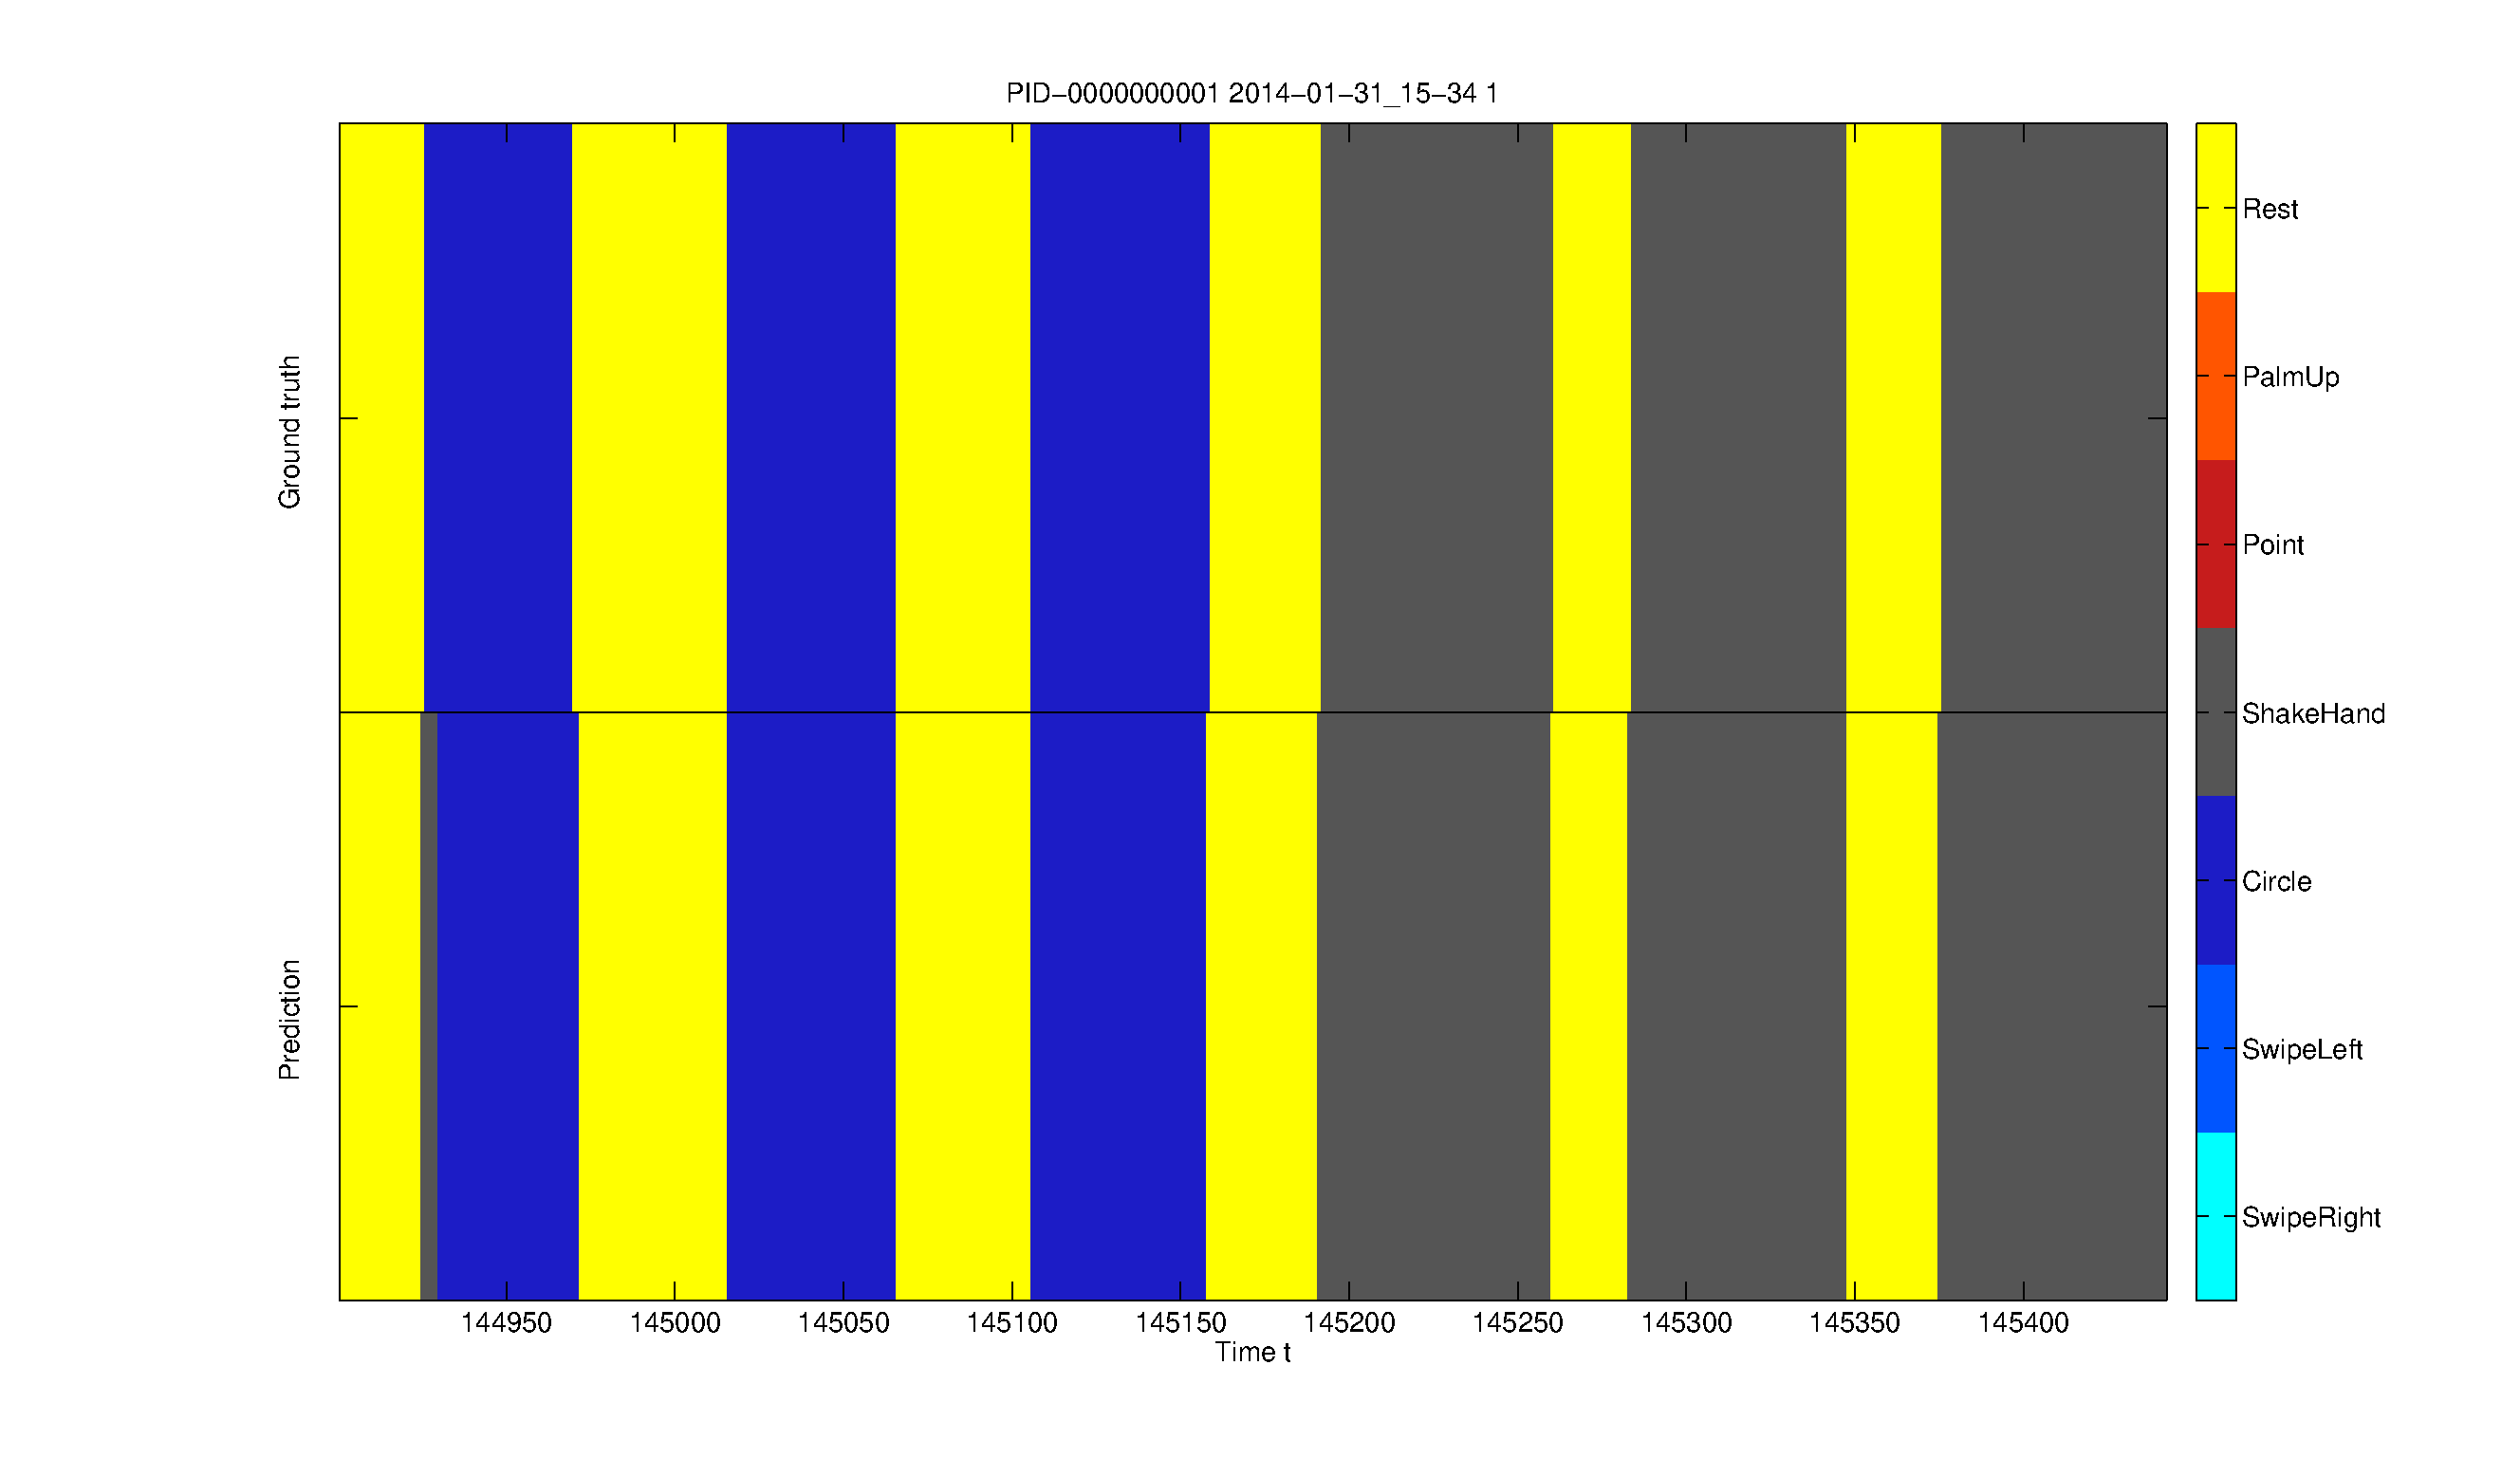
\includegraphics[width=\columnwidth]{fig/circle_shake.eps}
\caption{Visualization of recognition result.}
\label{fig:visual_recog}
\end{figure}

\begin{figure}[t]
\centering
\includegraphics[width=\columnwidth]{fig/circle_shake_label.ps}
\end{figure}

Fig.~\ref{fig:visual_recog} shows a visualization of the recognition result on a
test sequence.

\section{User Study and Data Collection}
As mentioned in Related Work, there is a lack of gesture data set that
includes both gestures with distinct paths and gestures with distinct hand
poses. To evaluate our method, we collected a dataset with the two forms of
gestures mentioned in Section~\ref{sec:taxonomy}.

A vocabulary of 7 one-hand/arm gestures focusing on combining two \textit{forms}
gestures has been chosen. The gestures are also chosen based on possible
application in gesture-controlled PowerPoint presentation. The vocabulary has
been chosen to span over different potential difficulties (see the comments in
Table~\ref{tab:gestures}).

\begin{table}
\caption{}
\label{tab:gestures}
\centering
\begin{tabular}{|c|l|l|l|}
\hline
\# & Name of gesture & Form & Comment \\
\hline
1 & Swipe left & distinct path & simple path \\
\hline
2 & Swipe right & distinct path & simple path \\
\hline
3 & Circle & distinct path & complex path \\
\hline
4 & Horizontal wave & distinct path & has arbitrary repetitions \\
\hline
5 & Point & distinct hand pose & arbitrary path \\
\hline
6 & Palm forward & distinct hand pose & arbitrary path \\
\hline
7 & Grab & distinct hand pose & arbitrary path \\
\hline
\end{tabular}
\end{table}

The dataset contains data from 12 paid participants (nine were female) each
doing 4 sessions. All the participants are university students.
The participants were shown video demonstration of each gesture at the beginning. In each
session, the participant performs each gesture class 3 times according to the
text prompts on screen indicating the name of the gesture to perform.
The order of the gesture is random and the time between each gesture is random
between 2s-6s. The first 2 sessions have ``Rest'' prompt between each gesture
telling participants to go to the rest position (hands relaxing at the side of
the body), and the second 2 sessions do not have ``Rest'' prompt so participants
can choose to rest or not between consecutive gestures. This is also an
additional challenge to previous datasets \cite{Ruffieux2013} where gestures are always
delimited by rest positions.

Unlike Ruffieux et al. \cite{Ruffieux2013}, we do not show video demonstration
every time the participant performs a gesture because we want to simulate more
realistic scenario. In real practice, it is unlikely that a user will follow a
video demonstration every he/she does a gesture. The result of this is that
there will be more variations among the participants.

To simulate arbitrary movement for gestures with distinct hand poses that
require continuous response, the text prompt also asks participants to draw
letters in the air with the specified hand poses. We did this because in the
pilot study, we found that with no actual task to perform and visual feedback,
the participants may feel uncomfortable to move arbitrarily.

The full corpus contains 
\begin{align*}
10P \times 4S \times 7G \times 3R = 840 \text{ gesture occurrences}
\end{align*}
where P = participants, S = sessions, G = unique gestures, R = repetitions per
gesture. It is approximately 96 minutes of continuous recording. The data
recorded is the raw data from the Kinect sensor including RGB, depth and
skeleton data.

\subsection{Qualitative Observations}
We find that there is considerable variations in the way participants perform
each gesture each they were give the same demonstration video. Variations are
observed in speed, the magnitude of motion, the paths and hand poses among other
aspects.

For example, some participants do swipe left and right in a rather straight
horizontal line, while others have a more curved path. Some participants start
the circle gestures at the bottom while others start at the top. Some
participants do swipe left and right with palm forward pose while others have
less distinct hand pose (hand is more relaxed). However within users, they are
quite consistent within each gesture. 

\subsection{User Preferences}
We also did a questionnaire with the 12 participants regarding gesture input
related questions. 

\begin{itemize}
  \item Predefined vs. user defined gestures: 90\% of the participants prefer to
  be able to define their own gestures if necessary while 10\% of them prefer to following prefined
gestures completely. No one prefers to define their own gestures out right either.
\item How to define gestures: 80\% prefers to giving examples to the system by
performing the gestures themselves; no one prefers to defining some rules in
terms of positions and directions of movement of the hands alone. However 20\%
prefers to being able to do both.
\item Number of repetitions per gesture for training: 50\% are willing to give a
maximum of 4 - 6 examples, 40\% are willing ot give 1 - 3 examples, and 10\% are
willing to give more than 13 examples. So average maximum is about 5
repetitions.
\item Number of gestures for an application: 80\% think 6-10 gestures are
appropriate and easy to remember for a given application, 20\% think 1 - 5.
\item Intuitiveness of the gesture vocabulary for PowerPoint presentation:
average score 4 / 5.
\end{itemize}

\subsubsection{Implication to Gesture Interaction Interface}
Based on our observation of large variation between users and small variations
within users and majority of participants preferring defining their own gestures
if necessary, it suggests that it may be more important to optimize user
dependent recognition. As no one prefers to define own gesture at the very
beginning, it also suggest that having a reasonable predefined gesture set and
base user independent model for recognition is useful too.

Recognition method based on examples will allow users to train models of their
own gestures easily and we also need to optimize for developing methods that
require a few number of examples.

\section{Performance Metric}
Both frame \cite{song12} (check) and event-based \cite{guyon13} metrics has been
used for evaluating gesture recognition system. Many of the performance metrics are more relevant for
offline applications such as video analysis and retrieval. Frame error based
metric can suffer from class skew problem \cite{ward11}. Frame-based metric is
less relevant for gestures requiring discrete response. Discrete response is
inherently event based, especially for online recognition, it is hard to
recognize the gesture at an earlier stage. Guyon et al.
\cite{guyon13} use Levenshtein distance between the ordered list of
recognized events and the ground truth events for the ChaLearn
Gesture Challenge 2012. Event-based metrics that ignore timing of the
recognition such as the one used in \cite{guyon13} is also lacking for real-time
applications where responsiveness of the system matters and hence the timing of
the recognition matters.

Ruffieux et al. proposed a time-base metric \cite{Ruffieux2013} in addition to
event-based metrics. In computing the event-based metrics, they only consider an
event ``correct'', if the absolute difference between start time of the
recognized nucleus phase and that of the ground truth nucleus phase, and the
absolute difference between the end time of the recognized nucleus phase and
that of the ground truth are both less than 50\% of the duration of the grounth truth
nucleus. As both the event based and the time based metrics take timing into
consideration, it is actually more difficult to compare different algorithms and
the choice of the 50\% of the grounth truth duration is somewhat arbitrary. We
propose to completely separate the time-based metrics and the event-based
metrics.

Ward et al. \cite{ward11} proposed a comprehensive hybrid
scheme by combining information from both frame and event scoring. compare
\cite{Ruffieux2013} and \cite{ward11}, emphasize one real-time and discrete response and responsiveness.

We also take a hybrid approach based on the the different types of system
response according to different flow of the gestures. continuous response,
fragment error not relevant for discrete response gesture.

\section{Experimental Evaluation}

Compare HOG feature from depth and color images

Compare using vs not using PCA and number of PCA components

Compare number of hidden states for different gesture phase

Compare different number of mixtures

Compare user dependent vs user independent result
Most users like to define their own gestures, then use user dependent evaluation

\section{Discussion}
% An example of a floating figure using the graphicx package.
% Note that \label must occur AFTER (or within) \caption.
% For figures, \caption should occur after the \includegraphics.
% Note that IEEEtran v1.7 and later has special internal code that
% is designed to preserve the operation of \label within \caption
% even when the captionsoff option is in effect. However, because
% of issues like this, it may be the safest practice to put all your
% \label just after \caption rather than within \caption{}.
%
% Reminder: the "draftcls" or "draftclsnofoot", not "draft", class
% option should be used if it is desired that the figures are to be
% displayed while in draft mode.
%

% Note that IEEE typically puts floats only at the top, even when this
% results in a large percentage of a column being occupied by floats.


% An example of a double column floating figure using two subfigures.
% (The subfig.sty package must be loaded for this to work.)
% The subfigure \label commands are set within each subfloat command, the
% \label for the overall figure must come after \caption.
% \hfil must be used as a separator to get equal spacing.
% The subfigure.sty package works much the same way, except \subfigure is
% used instead of \subfloat.
%
%\begin{figure*}[!t]
%\centerline{\subfloat[Case I]\includegraphics[width=2.5in]{subfigcase1}%
%\label{fig_first_case}}
%\hfil
%\subfloat[Case II]{\includegraphics[width=2.5in]{subfigcase2}%
%\label{fig_second_case}}}
%\caption{Simulation results}
%\label{fig_sim}
%\end{figure*}
%
% Note that often IEEE papers with subfigures do not employ subfigure
% captions (using the optional argument to \subfloat), but instead will
% reference/describe all of them (a), (b), etc., within the main caption.

% Note that IEEE does not put floats in the very first column - or typically
% anywhere on the first page for that matter. Also, in-text middle ("here")
% positioning is not used. Most IEEE journals/conferences use top floats
% exclusively. Note that, LaTeX2e, unlike IEEE journals/conferences, places
% footnotes above bottom floats. This can be corrected via the \fnbelowfloat
% command of the stfloats package.

\section{Conclusion}

% use section* for acknowledgement

% trigger a \newpage just before the given reference
% number - used to balance the columns on the last page
% adjust value as needed - may need to be readjusted if
% the document is modified later
%\IEEEtriggeratref{8}
% The "triggered" command can be changed if desired:
%\IEEEtriggercmd{\enlargethispage{-5in}}

% references section

% can use a bibliography generated by BibTeX as a .bbl file
% BibTeX documentation can be easily obtained at:
% http://www.ctan.org/tex-archive/biblio/bibtex/contrib/doc/
% The IEEEtran BibTeX style support page is at:
% http://www.michaelshell.org/tex/ieeetran/bibtex/
\bibliographystyle{IEEEtran}
% argument is your BibTeX string definitions and bibliography database(s)
\bibliography{IEEEabrv,main}
%
% <OR> manually copy in the resultant .bbl file
% set second argument of \begin to the number of references
% (used to reserve space for the reference number labels box)
% \begin{thebibliography}{1}
% 
% \bibitem{IEEEhowto:kopka}
% H.~Kopka and P.~W. Daly, \emph{A Guide to \LaTeX}, 3rd~ed.\hskip 1em plus
%   0.5em minus 0.4em\relax Harlow, England: Addison-Wesley, 1999.
% 
% \end{thebibliography}




% that's all folks
\end{document}


